  % vim: set ts=4 sw=4 ai et tw=74:
\documentclass[12pt,a4paper,portuges]{style/myreport}
\usepackage[portuges]{babel}
\usepackage[utf8]{inputenc}

%%%%%%%%%%%%%%%%%%%%%%%%%%%%%%%%%%%%% DADOS DA CAPA DO RELATÓRIO %%%%%%%%%%%%%%%%%%%%%%%%%%%%%%%%%%%%%%5
\newcommand{\AnoLectivo}{Ano Lectivo de 2010/11}
\newcommand{\TituloProjecto}{Planeta XPTO, Fase Final}
\newcommand{\NomeDaCadeira}{Disciplina de Computação Gráfica}
\newcommand{\Curso}{Licenciatura em Engenharia Informática}

\newcommand{\PrimeiraListaNomes}{António Cascais, Fábio Costa, Gabriel Poça, José Teixeira, Miguel Palhas}

\newcommand{\PrimeiroElemento}{54744 - António Carlos Pinheiro Cascais}
\newcommand{\SegundoElemento}{54822 - Fábio Rafael Costa}
\newcommand{\TerceiroElemento}{56974 - Gabriel Gonçalves Poça}
\newcommand{\QuartoElemento}{54749 - José António Teixeira}
\newcommand{\QuintoElemento}{54767 - Miguel Branco Palhas}
%%%%%%%%%%%%%%%%%%%%%%%%%%%%%%%%%%%%% FIM %%%%%%%%%%%%%%%%%%%%%%%%%%%%%%%%%%%%%%5

\usepackage[T1]{fontenc}
\usepackage{a4wide}
\usepackage{txfonts}% use Arial && Times New Roman
\usepackage[pdftex]{color,graphicx}
\usepackage{fancyhdr}
\usepackage{fancyvrb}
\usepackage{acronym}
\usepackage{cite}
\usepackage{longtable}
\usepackage{datetime}
%\usepackage{amssymb}
\usepackage[pdfauthor={\PrimeiraListaNomes},%
            pdftitle={\{\TituloProjecto\}},%
            urlcolor=darkblue,%
            citecolor=darkblue,%
            filecolor=darkblue,%
            linkcolor=darkblue,%
            pdftex,colorlinks,a4paper]{hyperref}
\definecolor{darkblue}{rgb}{0,0,0.6}
%\definecolor{darkred}{rgb}{0.8,0,0}

%%%%%%%%%%%%%%%%%%%%%%%%%%%%%%%%%%%% PACOTES PARA ADICIONAR CODIGO FONTE %%%%%%%%%%%%%%%%%%%%%%%%%%%%%%%%%%%%%%
\usepackage{listings}
\usepackage{color}
\usepackage{textcomp}
\definecolor{listinggray}{gray}{0.9}
\definecolor{lbcolor}{rgb}{0.9,0.9,0.9}
\lstset{
	%backgroundcolor=\color{lbcolor},   					% COR DE FUNDO
	tabsize=4,
	rulecolor=,
	language=c,								% TIPO DE LINUGAGEM DE PROGRAMAÇÃO
        basicstyle=\scriptsize,
        upquote=true,
        aboveskip={1.5\baselineskip},
        columns=fixed,
        showstringspaces=false,
        extendedchars=true,
        breaklines=true,
        prebreak = \raisebox{0ex}[0ex][0ex]{\ensuremath{\hookleftarrow}},
        %frame=single,								% LINHA QUE CONTORNA O CODIGO
        showtabs=false,
        showspaces=false,
        showstringspaces=false,
        identifierstyle=\ttfamily,
        keywordstyle=\color[rgb]{0,0,1},
        commentstyle=\color[rgb]{0.133,0.545,0.133},
        stringstyle=\color[rgb]{0.627,0.126,0.941},
}

%%%%%%%%%%%%%%%%%         UTILIZAÇÃO:
%%%%%%%%%%%%
%%%%%%%%%%                  Imprimir com uma linha à volta do código
%%%%%%%%%%                       \begin{lstlisting}[frame=single]
%%%%%%%%%%
%%%%%%%%%%                  Imprimir normalmente:
%%%%%%%%%%                       \begin{lstlisting}
%%%%%%%%%%                           #include <SDL.h>
%%%%%%%%%%                       \end{lstlisting}
%%%%%%%%%%
%%%%%%%%%%                  Imprimir Ficheiro:
%%%%%%%%%%                       \lstinputlisting{filename.java}
%%%%%%%%%%%%
%%%%%%%%%%%%%%%%%%%%%%%%%%%%%%%%%%%% FIM %%%%%%%%%%%%%%%%%%%%%%%%%%%%%%%%%%%%%%

%%%%%%%%%%%%%%%%%%%%%%%%%%%%%%%%%%%% COMO ADICIONAR IMAGENS NO RELATÓRIO %%%%%%%%%%%%%%%%%%%%%%%%%%%%%%%%%%%%%%
%%%%%%%%%%%%%%
%                 \begin{figure}[here]
%                 \centering{\includegraphics[width=0.5\textwidth]{images/1imagem.png}}
%                 \caption{Prototipo de imagem}
%                 \label{fig:prototype}
%                 \end{figure}
%
%                 Please see Figure ~\ref{fig:prototype} for a prototype blah blah blah
%%%%%%%%%%%%%%
%%%%%%%%%%%%%%%%%%%%%%%%%%%%%%%%%%%% FIM %%%%%%%%%%%%%%%%%%%%%%%%%%%%%%%%%%%%%%

\pdfpagewidth=\paperwidth
\pdfpageheight=\paperheight

\renewcommand\familydefault{\sfdefault}% usar font sem serifas


%%%%%%%%%%%%%%%%%%%%%%%%%%%%%%%%%%%%% HEADER das paginas %%%%%%%%%%%%%%%%%%%%%%%%%
\pagestyle{fancy}

\fancyhead[LO,RE]{\footnotesize \slshape \rightmark}
\fancyhead[LE,RO]{\footnotesize \slshape \leftmark} 
%\fancyfoot{}
%\fancyfoot[LO,RE]{\thepage}

%%%%%%%%%%%%%%%%%%%%%%%%%%%%%%%%%%%% FIM %%%%%%%%%%%%%%%%%%%%%%%%%%%%%%%%%%%%%%

% definir acrónimos com itálico
%\renewcommand*{\acf}[1]{\acffont{\textit{\acl{#1}}~\acfsfont{(\acs{#1})}}}

\newtheorem{defin}{Definição}

%\pagestyle{fancy}
%\lhead{}
%\rhead{}

\newenvironment{comando}
{\medskip
\begin{tt}}
{\end{tt}
\medskip}

\parindent=0pt
\parskip=4pt

%
% Commands and environments
%
%% vim: set ts=4 sw=4 ai et:

% insere uma imagem com legenda, por omissao com 12cm de largura
\newcommand{\image}[3][12cm]
{
    \begin{figure}[!h]
        \begin{center}
            \includegraphics[width=#1]{images/#2}
                \caption{#3}
                \label{fig:#2}
        \end{center}
    \end{figure}
    % force dump image queue here
    %\clearpage
}


\begin{document}

%% Capa Principal %%%%%%%%%%%%%%%%%%%%%%%%%%%%%%%%%%%%%%%%%%%%%%%%%%%%%%%
\thispagestyle{empty}

\setlength{\unitlength}{1cm}
\begin{picture}(0,0)

\put(14,0){\line(0,-1){24.5}}
\put(0,-12.2){\line(1,0){18}}
\put(0,-16.2){\line(1,0){18}}
\put(0,-12.2){\line(0,-1){4}}

\put(14.5,-3){
\includegraphics[height=2cm]{style/images/um}}
\put(14.5,-6){
\includegraphics[height=2cm]{style/images/eng}}
\put(14.5,-9){
\includegraphics[height=2cm]{style/images/di}}

\begin{minipage}[t]{16cm}
 
~

\addvspace{4cm}

Universidade do Minho

Conselho de Cursos de Engenharia

\Curso

\bigskip

{\Large \textbf{\NomeDaCadeira}}

\medskip

\AnoLectivo

\addvspace{7cm}

{\LARGE \ \TituloProjecto}

\addvspace{2.5cm}

\textbf{\PrimeiraListaNomes}

Grupo 26

\addvspace{0.5cm}

%
% Supervisão:  {\textless}{\textless}Orientador{\textgreater}{\textgreater}

\addvspace{2.5cm}

{\large \monthname, \newdateformat{dashdat}{\THEYEAR} \dashdat\today}

\end{minipage}
\end{picture}

\newpage

%% Segunda página %%%%%%%%%%%%%%%%%%%%%%%%%%%%%%%%%%%%%%%%%%%%%%%%%%%%%%%
\thispagestyle{empty}

\begin{flushright}
\begin{tabular}{|p{4cm}|p{4cm}|}
\hline
Data de Recepção & \\
\hline
Responsável & \\
\hline
Avaliação & \\
\hline
Observações & \\
& \\
& \\
\hline
\end{tabular}
\end{flushright}

~

\addvspace{8.4cm}

{\LARGE \textbf{ \TituloProjecto }}

\addvspace{2.5cm}

\textbf{\PrimeiroElemento}

\bigskip

\textbf{\SegundoElemento}

\bigskip

\textbf{\TerceiroElemento}

\bigskip

\textbf{\QuartoElemento}

\bigskip

\textbf{\QuintoElemento}

\addvspace{1.5cm}

{\large \monthname, \newdateformat{dashdate}{\THEYEAR} \dashdate\today}

\newpage

%% Página de dedicatória (opcional) %%%%%%%%%%%%%%%%%%%%%%%%%%%%%%%%%%%%%
%\thispagestyle{empty}

%{\textless}{\textless}Dedicatória{\textgreater}{\textgreater}

%\newpage

%% Resumo e Índices %%%%%%%%%%%%%%%%%%%%%%%%%%%%%%%%%%%%%%%%%%%%%%%%%%%%%
\pagenumbering{roman}
%% vim: set ts=4 sw=4 ai et tw=74:
\chapter*{Resumo}
\addcontentsline{toc}{chapter}{Resumo} 


% indices
%\renewcommand{\contentsname}{Índice}
\tableofcontents
\addcontentsline{toc}{chapter}{\contentsname}

%\renewcommand{\listfigurename}{Índice de Figuras}
\listoffigures
\addcontentsline{toc}{section}{\listfigurename}

%%%%%%%%%%%%%%%%%%%%%%%%%%%%%%%%%%%% LISTA DE TABELAS %%%%%%%%%%%%%%%%%%%%%%%%%%%%%%%%
%\renewcommand{\listtablename}{Índice de Tabelas}
%\listoftables
%\addcontentsline{toc}{section}{\listtablename}

\newpage

%% Texto normal %%%%%%%%%%%%%%%%%%%%%%%%%%%%%%%%%%%%%%%%%%%%%%%%%%%%%%%%%
\pagenumbering{arabic}

%% TODO: uncomment chapters


\chapter{Introdução}
À descoberta, digamos que esse foi o lema de todo o desenvolvimento, desde os requisitos obrigatórios aos extras, como o skybox, o salto, as animações, etc. Terminamos com algo cuja imagem fala por si, o jogo é simples, aos requisitos acrescentamos as árvores, de referir também as colisões com árvores e torres, a possibilidade de saltar, e assim evitar as balas, o céu, as animações, as imagem das vidas, o full screen, isto.
A de implementação contamos com o documento de configuração \textit{.ini}, o md2loader, profilling, entre outros.


\newpage

\chapter{Considerações Inicias}
% 
%%terreno plano v
%%dois tipos de camara v
%%aleatoriedade e radar v
%%modelos importados e formato v
%%uma unidade em OpenGL corresponde a 0.1metros v

Existem algumas considerações iniciais a ter em conta.

São enunciadas várias dimensões,distâncias, em metros. Visto que em OpenGL não se realizam medições em metros foi necessário encontrar uma forma de relacionar as medidas do OpenGL com as medidas pedidas.
Assim, para que seja possível criar o jogo de acordo com as medidas pedidas no enunciado, considerámos que 1 metro corresponde a 4 unidades em OpenGL.

Quanto ao terreno, é pedido que seja plano com 4km quadrados de área. Utilizando texturas foi suficiente arranjar uma imagem de acordo com o pretendido e gerar o plano através dela.

Em termos de jogabilidade é necessária a implementação de dois modos de câmara: \textit{Third Person Shooter} (tps) e outra \textit{First Person Shooter} (fps).
Alternar entre estes dois modos é feito através de uma tecla pré-definida.

O radar não indica a direcção em que está a chave e tem um raio de acção limitado a 500 metros.

Por ultimo são necessário alguns modelos para as torres, chaves, herói, etc. Por opção, estes modelos são do formato \textit{.md2}. Adiante será desenvolvido este ponto e explicada esta escolha.


\newpage


% ------------------ MODELOS
\chapter{Modelos}
% vim: set ts=4 sw=4 ai et tw=74:

%\addcontentsline{toc}{section}{Desenho do Sistema}

%dizer que modelos importamos e em que formatos
%%dizer porque e que escolhemos esses formatos
%codigo

Carregar objectos no mundo, ou melhor, modelos para objectos, foi um dos grandes desafios. Tanto pela limitação da disponibilidade gratuita, como pelas limitações do carregamento dos modelos, do tipo \textit{obj}, que nos foram inicialmente apresentados.

Modelos \textit{obj} não são carregados com textura de origem, ou seja, o uso de texturas implicaria a implementação da funcionalidade. Em acréscimo nas limtações está a ausência de animações.
Neste contexto surgiu \textit{md2}, um formato original do motor do jogo quake.

\textit{MD2} é um formato abundante e bastante frequente existindo ainda uma ferramenta que facilita o carregamento para opengl, o {\bf md2loader}.

No jogo são carregados sobre a forma de modelos \textit{md2} os seguintes objectos:
\begin{itemize}
\item Player;
\item Torres;
\item Balas;
\item Chaves;
\item Edifício do Tesouro.
\end{itemize}



\newpage

\section{MD2 Loader}


Uma das ferramentas externas da qual o projecto faz uso é o {\bf md2loader}.

O md2loader é uma ferramenta de código aberto que facilmente adaptamos às nossas necessidades. Em palavras simples, existe uma classe denominada \textit{MD2Player} que permite carregar um modelo md2 e realizar operações simples como definir a escala ou render do modelo. Depois de conhecido o processo foi simples criar uma classe própria para trabalhar com a ferramenta.

\-

\begin{figure}[h]
\begin{center}
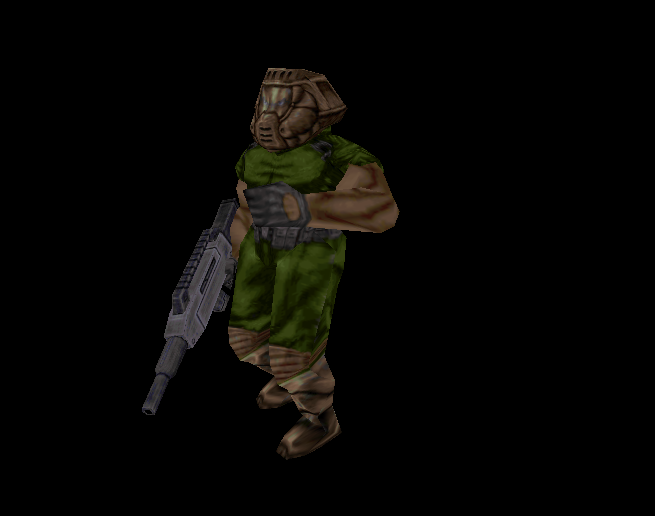
\includegraphics[width=0.5\textwidth]{images/md2loader.png}
\caption{Screenshot da ferramenta md2loader.}
\end{center}
\end{figure}





\newpage

\section{Player}

O player é aquele que se denomina ``herói'' do jogo. Ainda que nos seja permitido carregar qualquer modelo \textit{md2} optamos pela famosa figura dos jogos electrónicos, \textit{Sonic}.

Para controlar o player criamos uma classe, \textit{Player.cpp}.
Os modelos \textit{md2} utilizados suportam animações por frames. Assim, foi criada a classe Frame para gerir através da função \textbf{glutTimerFunc} o incremento das frames num intervalo fixo de tempo, configurável no ficheiro \textbf{config.ini}. Isto faz com que a cada intervalo, a frame actual seja incrementada, e quando o jogador está em movimento estas alternem ciclicamente, criando a ilusão de movimento.

\-
\begin{tabular} {l | p{10cm}}
\begin{lstlisting}
class Player : public Model_MD2 {
public:
	Frame *anim;
	float ang_x, ang_y;
	float speed_front, speed_back, speed_side;
	float speed_rotate_x, speed_rotate_y;
	float wall_dist;
	bool isJumping;
	int jump_time;
	int jump_max;
	bool canJump;
	int jump_cooldown;
	int tower_colision_dist;
	int tree_colision_dist;

	GameState state;

	Player(const std::string &path);

	void move(Vertex *new_coords);
	bool isMoving();
	void update();
	void render();

	float jumpOff(int off);

	static void inc_frame(int val);

	void calcColisions();
};
\end{lstlisting} 
&
Header da classe Player.cpp .\\
\end{tabular}

\subsection{Modos de Câmera}
% vim: set ts=4 sw=4 ai et tw=74:

%\addcontentsline{toc}{chapter}{Lista de Acrónimos}

%Falar dos dois tipos de camaras
%Tecnicas para a implementaçao destes tipos
%como mudar entre as camaras
%codigo

A câmera é posicionada no mundo relativamente ao posicionamento e direcção do jogador. são implementados dois modos de visualização.
Em termos práticos, o cálculo da posição da câmara consiste em cálculos a partir dos vectores de posição e direcção do jogador, com alguns ajustes para um melhor posicionamento. Isto depende, obviamente do tipo de câmara utilizada:

\begin{description}
\item[Terceira Pessoa] Câmara colocada atrás do modelo ligeiramente acima e com a direcção do modelo. Ao vector de posição do jogador, é subtraido o seu próprio vector de direcção multiplicado por um factor de distância, para colocar a câmara nas costas do jogador. Há ainda um ajuste na coordenada Y para câmara ficar ligeiramente acima do jogador e ser possivel ver o que está para a frente deste. É também feito um teste para impedir que a câmara se posicione abaixo do nivel do terreno.
\item[Primeira Pessoa] Câmara colocada em frente ao modelo com a direcção do modelo. O método de calculo é semelhante ao anterior, apenas muda a equaçao, para posicionar a câmara á frente do jogador, em vez de nas suas costas.
\end{description}

Para ficar mais claro, eis o código de cálculo da posição da câmara:

\begin{lstlisting}[caption=Função de posicionamento da câmara]
void Camera::placeCamera() {
	Vertex* pos = g_player->coords;
	Vertex* dir = g_player->direction;

	glLoadIdentity();

	int cam_mode = InputManager::getOpState(CAMERA_MODE);

	if (cam_mode == KEY_OFF) {
		int tps_off = conf.rint("camera:tps_off");
		int tps_y_off = conf.rint("camera:tps_y_off");
		int tps_dir_y_off = conf.rint("camera:tps_dir_y_off");

		camPos->x = pos->x - tps_off * dir->x;
		camPos->z = pos->z - tps_off * dir->z;
		camPos->y = max(pos->y - tps_off * dir->y + tps_y_off, g_map->triangulateHeight(camPos->x, camPos->z) + terrain_offset);

		camDir->x = pos->x;
		camDir->y = pos->y + tps_dir_y_off;
		camDir->z = pos->z;
	} else {
		int fps_off = conf.rint("camera:fps_off");
		int fps_y_off = conf.rint("camera:fps_y_off");
		int fps_dir_y_off = conf.rint("camera:fps_dir_y_off");

		camPos->x = pos->x + fps_off * dir->x;
		camPos->z = pos->z + fps_off * dir->x;
		camPos->y = max(pos->y + fps_y_off, g_map->triangulateHeight(camPos->x, camPos->z));

		camDir->x = pos->x + (fps_off + 1) * dir->x;
		camDir->y = pos->y + dir->y + fps_dir_y_off;
		camDir->z = pos->z + (fps_off + 1) * dir->z;
	}


	gluLookAt(camPos->x, camPos->y, camPos->z,
		camDir->x, camDir->y, camDir->z,
		0, 1, 0);
}

\end{lstlisting} 

O código começa por saber as coordenadas e direcção do jogador, e conforme o tipo de câmara seleccionado (a câmara pode ser alternada pela tecla 'C'), calcula as posições da câmara, terminando então com a chamada ao \textbf{gluLookAt}.


\newpage

\section{Torres e Keys}
Para a gestão das torres e das existem duas classes, \textit{Towers.cpp} e \textit{Keys.cpp} respectivamente.

\-
\begin{center}
\begin{tabular} {l | p{10cm}}
\begin{lstlisting}[caption=Cabeçalho da classe Keys]
class Keys {
public:
    int num_keys, catched_count;
    float catch_dist;
    Key **keys;

    Keys();

    void render();
    void update();
    int get_closest_distance();
};
\end{lstlisting} 
& 
Header da classe Keys.cpp .
\end{tabular}
\end{center}
\-
Como se pode ver a classe keys é constituida por um array de instâncias da classe \emph{Key}, um numero de chaves (\emph{num\_keys}) que se encontra no documento config.ini e o numero de chaves apanhadas pela jogador (\emph{catched\_count}).
Existe ainda um método de update, que actualiza o modelo das chaves, determina se uma chave foi ou não apanhada, um método de render, que desenha as torres no mundo e por ultimo um método que calcula a distancia da chave que se encontra a menor distancia do jogador, inferior a 500 metros.

Para as torres o conceito é o mesmo, com a excepção do \emph{catched\_count} e do método \emph{get\_closest\_distance}.
No entanto as torres têm a caracteristaca de rodar na direcção do jogador quando este se encontra no seu alcance.

Na inicialização do jogo, são calculadas posições aleatórias para as chaves e torres. Estas posições têm em conta que uma torre ou chave nunca deverá ficar a menos de uma determinada distância (definida no ficheiro ini) de outra chave ou torre, evitando assim por exemplo, que uma chave fique escondida dentro do modelo de uma torre.

O algoritmo de cálculo da {\bf distancia entre dois modelos} é simples. Tendo as coordenadas do dos modelos temos:

\begin{center}
\begin{math}
Player => (a1,b1)
\end{math}
,
\begin{math}
Tower => (a2,b2)
\end{math}

\begin{equation}
Distancia = \sqrt{((a1-a2)^2+(b1-b2)^2)}
\end{equation}
\end{center}


\subsection{Angulo de orientação das Torres}

O angulo de orientação das torres para o player pode ser determinado fazendo uso do produto escalar entre dois vectores, a direção do player para a torre e o vector unitário (1,0,0). Sabemos que

\-
\begin{center}
\begin{math}
Player => (a_1,a_2)
\end{math}
,
\begin{math}
Tower => (b_1,b_2)
\end{math}

\begin{equation}
produto escalar = a_1*b_1 + a_2*b_2
\end{equation}
\begin{equation}
produto escalar = direccao * unitario * cos x
\end{equation}
\end{center}

Como tal, orientado em função do angulo \emph{x} temos:

\begin{equation}
x = acos( (a_1*b_1 + a_2*b_2 ) / direccao * unitario * cos x )
\end{equation}


Este angulo é a orientação que uma torre deve assumir para se orientar para um player, está claro, quando a distância é inferior ao alcance da torre.






\section{Edifício do Tesouro}
	O edifício do Tesouro é constituído por um arco-íris em torno de um objecto. O arco-íris é formado a partir de 7 \textit{torus}. É colocado no canto oposto do mapa, face à posição inicial do jagador, e serve como "meta final", onde o jogador se deve dirigir depois de recolhidas todas as chaves.


\begin{figure}[here]
                 \centering{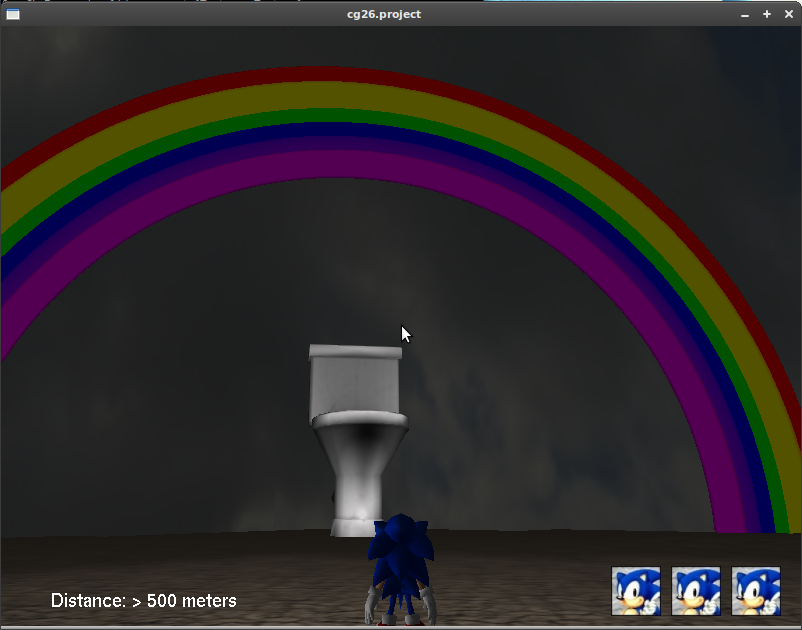
\includegraphics[width=0.5\textwidth]{images/tesouro.png}}
                 \caption{Edificio do tesouro.}
                 \label{fig:prototype}
\end{figure}


\newpage


 % ----------------- INI
\chapter{Ficheiro ini}


Um ponto relevante do projecto passa pelo ficheiro {\bf config.ini} . Neste documento estão todas as variáveis de uso frequente, ou melhor, todas as variáveis manipuláveis sem implicar recompilar o jogo, o que seria necessário para valores em \#define. Estes valores são "carregados"\ para o jogo quando necessário, mariotariamente no inicar do mesmo.

\-
\begin{center}
\begin{tabular} {l | p{10cm}}
\begin{lstlisting}
[game]
distance_factor		= 4
updates_per_second	= 60
anims_per_second	= 20
num_towers			= 15
num_keys			= 1
tower_range			= 1000
towers_min_distance = 500
\end{lstlisting} 
& 
Este é um exemplo de algumas configurações do jogo no documento {\bf config.ini}. \\
\end{tabular}
\end{center}

Este processo simplifica dois aspectos muito importantes. Para começar, possibilita a existência de um \emph{repositório} central com todos os valores usados ao longo do jogo. Por outro, facilita a alteração destes valores, o que ajuda bastante a efectuar pequenos ajustes no jogo sem ter a necessidade de recompilar o programa (processo que, como se constatou, tornou-se bastante longo á medida que o tamanho do código foi crescendo).

Eis de seguida um exemplo da utilidade desta classe, neste caso na criação da instância do jogador:

\begin{lstlisting}
Player::Player(const string &path) : Model_MD2(path) {
	state = GAME_ON;
	coords = new Vertex();
	coords->x = GLManager::distance(conf.rfloat("player:x"));
	coords->z = GLManager::distance(conf.rfloat("player:z"));
	coords->y = g_map->triangulateHeight(coords->x, coords->z);
	direction = new Vertex(0, 0, 1);
	ang_x = 0;
	ang_y = M_PI / 2;
	md2_rendermode = 0;

	speed_front = GLManager::convertFromKmH(conf.rfloat("player:speed_front"));
	speed_back = GLManager::convertFromKmH(conf.rfloat("player:speed_back"));
	speed_side = GLManager::convertFromKmH(conf.rfloat("player:speed_side"));
	speed_rotate_x = conf.rfloat("player:speed_rotate_x");
	speed_rotate_y = conf.rfloat("player:speed_rotate_y");


	anim = new Frame();
	anim->add_anim(MOVE_NONE, conf.rint("player:stop_frame"), conf.rint("player:stop_frame_end"));
	anim->add_anim(MOVE_WALK, conf.rint("player:walk_frame"), conf.rint("player:walk_frame_end"));
	anim->add_anim(MOVE_JUMP, conf.rint("player:jump_frame"), conf.rint("player:jump_frame_end"));

	jump_max = conf.rint("player:jump_max");
	isJumping = false;
	jump_time = 0;
	canJump = true;
	jump_cooldown = conf.rint("player:jump_cooldown");

	tower_colision_dist = conf.rint("player:tower_colision_dist");
	tree_colision_dist = conf.rint("player:tree_colision_dist");
}
\end{lstlisting}

Como se pode ver, esta classe depende fortemente de valores registados no ini, que são aqui lidos através das funções \textbf{conf.rint} e \textbf{conf.rfloat}, demonstrando assim a utilidade deste processo.


\newpage

% ------------------ RADAR
\chapter{Radar}
O radar apresenta a distância à chave mais próxima num limite de 500 metros, valor que pode facilmente ser editado no ficheiro \textbf{config.ini}.
A informação é mostrada textualmente no ecrã. Quando todas as chaves são apanhadas, essa informação é reflectida no radar, que indica ao jogador que deve procurar o final.

\begin{figure}[here]
                 \centering{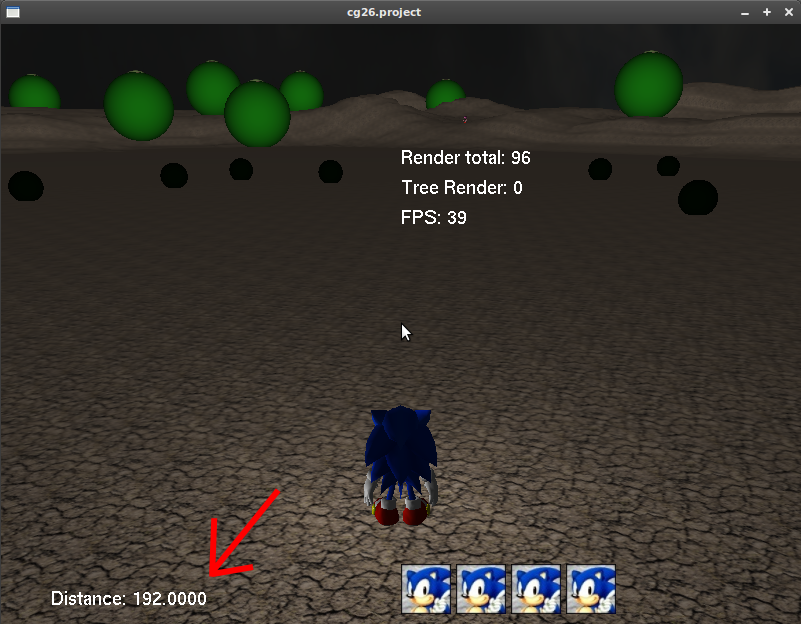
\includegraphics[width=0.9\textwidth]{images/radar.png}}
                 \caption{Radar.}
                 \label{fig:prototype}
\end{figure}


\newpage

% ------------------ INPUT
\chapter{Input}
O input é tratado através da classe InputManager. Esta classe mantém uma estrutura com o estado actual de todas as teclas utilizadas no jogo, bem como informação sobre as coordenadas e movimento do rato. Os eventos de pressionar ou libertar uma tecla apenas accionam um método que altera o estado da tecla correspondente na estrutura.

Assim, em qualquer ponto do código, é possivel saber o estado de uma tecla (pressionada ou não), e consoante essa flag, executar uma determinada acção. Esta estruturação permite uma gestão mais flexivel do input do que aquela utilizada nas aulas práticas, em que a função de gestão do input executava as próprias acções. Isto fazia com que a interacção fosse mais limitada, não sendo considerada a utilização de várias teclas ao mesmo tempo. Essa funcionalidade já é obtida por uma estrutura como a classe aqui utilizada.

Foi assim possivel implementar facilmente a utilização de várias teclas para ligar/desligar determinadas opções durante o decorrer do jogo:
\begin{itemize}
\item[C] Alternar entre os dois modos de câmera;
\item[M] Ligar/Desligar a música;
\item[N] Ligar/Desligar os restantes sons;
\item[F1] Activar o modo GL\_LINES da função {\textbf glPolygonMode} (para efeitos de Debug);
\item[F2] Desactivar o modo GL\_LINES;
\item[P] Activar/Desactivar o Profiling
\item[W,A,S,D] Movimentar o jogador pelo terreno;
\item[Espaço] Saltar;
\item[Rato] O movimento do rato traduz-se em movimento da câmara na direcção correspondente, e também da orientação do jogador no terreno;
\end{itemize}


\newpage	

% ------------------ MAPA DE ALTURAS
\chapter{Mapa de alturas e navegação}
O terreno de jogo deve ser criado de forma a possuir ligeiras elevações, e não ser apenas plano. Consequentemente, o posicionamento e navegação dos objectos pelo terreno deve acompanhar esta ondulação. Para implementar isto, foi usado um mapa de alturas, que consiste numa imagem em tons de cinza, onde cada pixel, de acordo com a sua tonalidade, representa uma altura.
Esse mapa é então escalado para corresponder ao número de pixeis necessários para gerar o terreno, e é feito um mapeamento entre cada pixel do terreno e a respectiva altura.

É aqui apresentado o código do carregamento da imagem usada como mapa de alturas:

\begin{lstlisting}
void Textures::loadHeightMap(string path, int width) {
	ilGenImages(1, &(textures[TERRAIN_HEIGHT].id));

	ilBindImage(textures[TERRAIN_HEIGHT].id);
	ilLoadImage(path.c_str());
	iluScale(width, width, 8);

	#ifndef rocket
	ilConvertImage(IL_LUMINANCE,IL_UNSIGNED_BYTE);
	#endif
	
	textures[TERRAIN_HEIGHT].w = ilGetInteger(IL_IMAGE_WIDTH);
	textures[TERRAIN_HEIGHT].h = ilGetInteger(IL_IMAGE_HEIGHT);
	textures[TERRAIN_HEIGHT].data = ilGetData();
}
\end{lstlisting}

A imagem é carregada com recurso á biblioteca DevIL, e é convertida para o formato \emph{IL\_LUMINANCE} para representar uma escala de cinzentos.

Com isto, é obtido um array com os dados da imagem a partir do qual se pode obter informação sobre a altura de cada vertice do mapa, da seguinte forma:

\begin{lstlisting}[caption=Função de cálculo da altura de um vértice do mapa]
float Map::map_h(int x, int z) {
	return this->heightMapData[x + this->tex_height.w * z];
	return 0;
}
\end{lstlisting}

Além de calcular a altura de cada vértice, é necessário calcular também a altura intermédia de cada ponto no interior dos triangulos do terreno, para proporcionar um movimento fluido. Para isto é feita uma interpolação com base nas alturas dos vértices adjacentes ao ponto que se pretende calcular:

\begin{lstlisting}[caption=Interpolação da altura de um ponto]
float Map::triangulateHeight(float x, float z) {
	double intX, intZ;
	float fracX, fracZ;

	x /= grid_width;
	z /= grid_width;

	fracX = modf(x, &intX);
	fracZ = modf(z, &intZ);

	float alt1, alt2;

	alt1 = this->map_h(intX, intZ) * (1 - fracZ) + this->map_h(intX, intZ + 1) * fracZ;
	alt2 = this->map_h(intX + 1, intZ) * (1 - fracZ) + this->map_h(intX + 1, intZ + 1) * fracZ;

	return alt1 * (1 - fracX) + alt2 * fracX;
}
\end{lstlisting}



% ------------------ DISPAROS
\chapter{Disparos}
As balas são objectos disparados por cada torre quando o jogador se aproxima da mesma.
Tem uma direcção fixa, que corresponde à direcção entre a torre e o jogador no momento do disparo, e viajam a uma velocidade superior á do jogador.
Para representar as balas, foram usados modelos MD2 animados, tal como para o jogador.

Em cada actualização do estado do jogo, é verificado se existe colisão entre o jogador e alguma das balas. Caso isso aconteça, o jogador perde uma vida (perdendo o jogo caso fique sem vidas).

Eis a função que testa a colisão entre uma bala e o jogador

\begin{lstlisting}
void Bullets::bullet_hit_test() {
    Vertex *c_bullet, *c_player = g_player->coords;
    for (list<Bullet>::iterator it = bullets.begin(); g_lifes->lifes > 0 && it != bullets.end(); it++) {
        c_bullet = it->coords;
        if (sqrt(pow(c_player->x - c_bullet->x, 2) + pow(c_player->y - c_bullet->y, 2) + pow(c_player->z - c_bullet->z, 2)) <= BULLET_HIT_DIST) {
            g_lifes->lifes--;
			it = bullets.erase(it);
        }
    }
}
\end{lstlisting}

A função calcula a distância entre as coordenadas da bala e do jogador. Se esta distância for menor que um determinado valor, houve colisão, e o número de vidas do jogador é decrementado, e a bala eliminada do jogo.

\newpage

% ------------------ FRUSTUM
\chapter{View Frsutum Culling}
\chapter{View Frsutum Culling}

Da teoria à prática, a maior dificuldade. De entre as diferentes abordagens, após alguma pesquisa, ficamos pela {\bf Geométrica}, pelo simples facto de não existir desvantagens notáveis face às restantes. Deste modo o View Frustum Culling está implementado para balas, torres e árvores.

\section{Bounding Spheres}
Está claro que \textit{axis aligned bounding boxes} é uma melhor implementação que \textit{bounding spheres} uma vez que permite criar uma menor margem de erro para casos de objectos no limite do frustum. No entanto trata-se de um jogo com poucos objectos onde a diferente margem de erro não será significativa e como tal \textit{bounding spheres} são a melhor escolha vez que apresentam o mesmo resultado e mais facil implementação.


\begin{lstlisting}[caption=Método para teste com \textit{bounding spheres}.]
int Frustum::sphereInFrustum(Vertex *p, float raio) {

    int result = INSIDE;
    float distance;

    for (int i = 0; i < 6; i++) {
        distance = pl[i].distance(p);
        if (distance < -raio)
            return OUTSIDE;
        else if (distance < raio)
            result = INTERSECT;
    }
    return (result);

}
\end{lstlisting}

\begin{figure}[here]
                 \centering{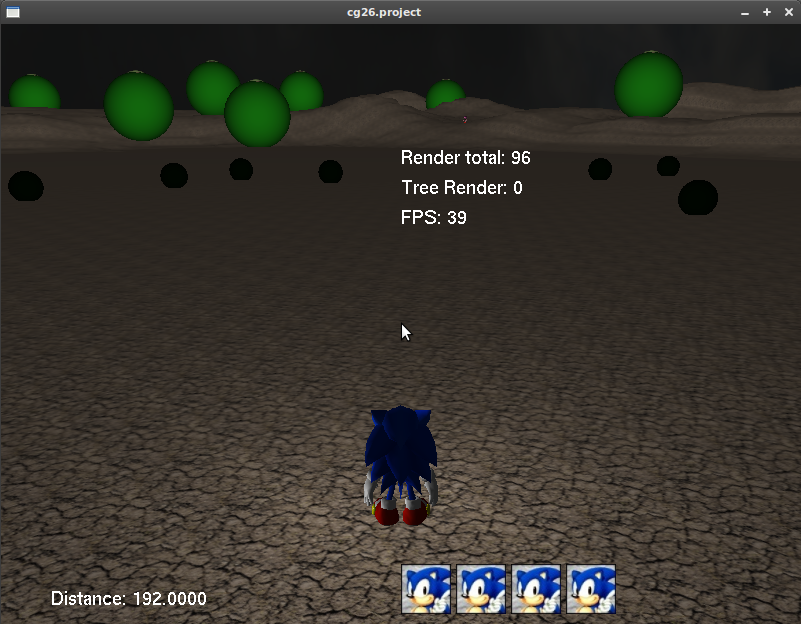
\includegraphics[width=0.8\textwidth]{images/frustum.png}}
                 \caption{Implementação de \textit{bounding spheres}.}
                 \label{fig:prototype}
\end{figure}

\newpage

% ------------------ PROFILLING
\chapter{Profilling}
\chapter{Profiling}
Ainda que um extra, ou talvez mesmo não um extra uma vez que é uma componente de desenvolvimento não de jogo, cramos também um modulo para profiling. Para efectuar os calculos existem três arrays para guardar a informação:

\begin{description}
\item[\textit{start}] Registo o tempo no inicio da medição.
\item[\textit{end}] Regista o tempo no final da medição.
\item[\textit{name}] Regista a descrição da medição.
\end{description}

A utilização é intuitiva. É invocado o método start\_time com um identificador e uma descrição, ou nome no inicio da medição e end\_time com o mesmo identificador no final da medição. Feito render é impresso para o ecrã a subtração entre tempo final e inicial associado à descrição.

\begin{lstlisting}
void start_time(int num, char* name);
void end_time(int num);
void render();
\end{lstlisting}



\newpage

% ------------------ VBO
\chapter{Vertex Buffer Objects}
Os Vertex Buffer Objects (VBOs) disponibilizam uma método de render mais eficiente para um conjunto de vértices estático. Através desta ferramenta é possível definir, na fase de inicialização do programa, um conjunto de vértices com todas as suas propriedades (coordenadas de textura, cores, normais) e armazená-los previamente num buffer na placa gráfica.

Neste projecto foram usados VBOs para o desenho do mapa de jogo, por ser o objecto que é estático ao longo de todo o decorrer do jogo. A sua implementação foi feita à custa da função Map::initVBO.

\begin{lstlisting}[caption=Cálculo dos buffers para VBOs (alocação)]
void Map::initVBO() {
	//float *vertexB, *texB, *normalB;
	int vertexSize = grid_n * grid_n * 3 * sizeof (float);
	int texSize = grid_n * grid_n * 2 * sizeof (float);
	int normalSize = grid_n * grid_n * 3 * sizeof (float);
	int stripSize = grid_n * 2 * sizeof (unsigned int);
	n_strips = grid_n - 1;

	//cria espaco temporario para preencher os buffers
	vertexB = (float *) malloc(vertexSize);
	texB = (float *) malloc(texSize);
	normalB = (float *) malloc(normalSize);
	grid_strips = (unsigned int **) malloc(sizeof (unsigned int *) * n_strips);
\end{lstlisting}
A função começa por reserver espaço temporário na memória principal para armazenar os buffers.

\begin{lstlisting}[caption=Cálculo dos buffers para VBOs (vértices)]
	//preencher o buffer de vertices
	float *vertexAux = vertexB;
	float *texAux = texB;
	for (int x = 0; x < grid_n; x++) {
		for (int y = 0; y < grid_n; y++) {
			vertexAux[0] = grid_width * x;
			vertexAux[2] = grid_width * y;
			vertexAux[1] = this->map_h(x, y);
			vertexAux += 3;

			texAux[0] = x;
			texAux[1] = y;
			texAux += 2;
		}
	}
\end{lstlisting}
De seguida são preenchidos os buffers com as coordenadas dos vértices, e respectivas coordenadas de textura.

\begin{lstlisting}[caption=Cálculo dos buffers para VBOs (normais)]
	float *normalAux = normalB;
	for (int x = 0; x < grid_n; x++) {
		for (int y = 0; y < grid_n; y++) {
			Vertex *N = (x == 0) ? vertexFromBuffer(vertexB, x, y) : vertexFromBuffer(vertexB, x - 1, y);
			Vertex *S = (x == grid_n - 1) ? vertexFromBuffer(vertexB, x, y) : vertexFromBuffer(vertexB, x + 1, y);
			Vertex *W = (y == 0) ? vertexFromBuffer(vertexB, x, y) : vertexFromBuffer(vertexB, x, y - 1);
			Vertex *E = (y == grid_n - 1) ? vertexFromBuffer(vertexB, x, y) : vertexFromBuffer(vertexB, x, y + 1);

			Vertex *normA = new Vertex(S->x - N->x, S->y - N->y, S->z - N->z);
			Vertex *normB = new Vertex(E->x - W->x, E->y - W->y, E->z - W->z);

			Vertex *norm = new Vertex(normA->y * normB->z - normA->z * normB->y,
				normA->z * normB->x - normA->x * normB->z,
				normA->x * normB->y - normA->y * normB->y);

			norm->normalize();

			normalAux[0] = -norm->x;
			normalAux[1] = -norm->y;
			normalAux[2] = -norm->z;
			normalAux += 3;
		}
	}
\end{lstlisting}
O cálculo das normais, por depender dos vértices adjacentes, não pode ser calculado em paralelo com os restantes, por isso é aqui feito isoladamente, recorrendo a um algoritmo que estima uma aproximação à normal com base nos 4 vértices ortogonalmente adjacentes.

\begin{lstlisting}[caption=Cálculo dos buffers para VBOs (índices)]
	//preenche as strips
	for (int x = 0; x < n_strips; x++) {
		grid_strips[x] = (unsigned int *) malloc(stripSize);
		unsigned int *stripAux = grid_strips[x];
		for (int y = 0; y < grid_n; y++) {
			stripAux[0] = y + (x + 1) * grid_n;
			stripAux[1] = y + x * grid_n;
			stripAux += 2;
		}
	}
\end{lstlisting}

Finalmente, são calculados os arrays dos índices indicando a ordem pela qual os vértices devem ser desenhados. O mapa fica dividido em strips pelo que deve ser gerado um array de índices por cada strip.

\begin{lstlisting}[caption=Cálculo dos buffers para VBOs (envio dos buffers)]
	//gera e envia os buffers
	glGenBuffers(MAP_BUFF_COUNT, buffers);

	glBindBuffer(GL_ARRAY_BUFFER, buffers[MAP_VERTEX]);
	glBufferData(GL_ARRAY_BUFFER, vertexSize, vertexB, GL_STATIC_DRAW);
	glVertexPointer(3, GL_FLOAT, 0, 0);

	glBindBuffer(GL_ARRAY_BUFFER, buffers[MAP_TEX]);
	glBufferData(GL_ARRAY_BUFFER, texSize, texB, GL_STATIC_DRAW);
	glTexCoordPointer(2, GL_FLOAT, 0, 0);

	glBindBuffer(GL_ARRAY_BUFFER, buffers[MAP_NORMAL]);
	glBufferData(GL_ARRAY_BUFFER, normalSize, normalB, GL_STATIC_DRAW);
	glNormalPointer(GL_FLOAT, 0, 0);

	//liberta os buffers temporarios
	free(texB);
	if (drawNormals == false) {
		free(vertexB);
		free(normalB);
	}
}
\end{lstlisting}

Para terminar, a função envia os buffers calculados para a placa gráfica, e liberta a memória temporária alocada no início.

O render do mapa passa então a ser um ciclo simples, invocando os arrays de strips aqui calculados:

\begin{lstlisting}[caption=Render do mapa com VBOs]
void Map::render() {
	int x = 0, y = 0;

	glBindTexture(GL_TEXTURE_2D, tex_soil.gl_id);

	glMaterialfv(GL_FRONT, GL_AMBIENT, mat_amb);
	glMaterialfv(GL_FRONT, GL_AMBIENT, mat_diff);
	glMaterialfv(GL_FRONT, GL_SPECULAR, mat_spec);

	for (int x = 0; x < n_strips; x++) {
		glDrawElements(GL_TRIANGLE_STRIP, grid_n * 2, GL_UNSIGNED_INT, grid_strips[x]);

	}

	glBindTexture(GL_TEXTURE_2D, 0);
}
\end{lstlisting}


% ------------------ DISPLAY LISTS
\chapter{Display Lists}
As display lists são, para além dos Vertex Buffer Objects e do View Frustum Culling, outro método de optimizar a aplicação. Podem ser vistas como a criação de listas de render pré-compiladas, que ficam armazenadas na placa gráfica. Deste modo, em vez de ser necessário a cada render, fazer sucessivas invocações a funções como \textbf{glVertex3f}, \textbf{glTranslatef}, etc, estas funções são chamadas apenas na inicialização dentro da definição de uma Display List, que é então compilada para a gráfica.
Durante o render apenas é necessário invocar a lista criada, através do seu identificador.

Neste projecto foram usadas Display Lists em vários pontos, e em algumas delas houve subtilezas que foi necessário ter em conta:
\begin{itemize}
\item[Torres] Foi criada uma Display List para representar uma torre. Como cada torre tem uma orientação diferente, que vai variando ao longo do jogo, não seria possivel criar uma Display List geral para fazer o render de todas as torres. Assim o render das torres resume-se a fazer a translação e rotação para o local correcto, seguido da invocação da DL.
\item[Árvores] Para as árvores já seria possivel definir, primeiro uma DL para uma árvore individual, e depois uma DL geral para o render de todas as árvores, á custa da primeira DL.
Porém isto também não foi implementado pois não permitiria aplicar o View Frustum Culling nas árvores, que revelou ser uma alternativa mais eficiente. Assim o método usado foi idêntico ao das torres, apenas com uma DL para uma árvore.
\item[Balas] As balas têm a particularidade de possuirem animações. No total cada bala alterna entre 7 frames diferentes. Ainda assim, foi notado que, criando uma DL para cada uma das frames, a performance da aplicação era melhorada. Isto foi particularmente interessante ao verificar-se que deste modo, passou a ser possivel ter centenas de balas animadas em simultâneo em jogo, e ainda manter um nível de FPS aceitavel.
\end{itemize}

Eis como exemplo, a geração e invocação da DL para as torres:

\begin{lstlisting}
void Towers::createTowerList() {
    md2_rendermode = 0;
    set_scale(conf.rfloat("game:tower_scale"));
	
	tower_list = glGenLists(1);
	glNewList(tower_list, GL_COMPILE);
	md2_model->drawPlayerItp(true, static_cast<Md2Object::Md2RenderMode> (0));
	glEndList();
}

void Tower::render() {
    if (g_frustum->sphereInFrustum(new Vertex(coords->x, coords->y + 36, coords->z), radius)) {
        glPushMatrix();
        glTranslatef(coords->x, coords->y, coords->z);
        glRotatef(90 + (ang_x * 180) / M_PI, 0, 1, 0);
        glCallList(g_towers->tower_list);
        glTranslatef(0, 37, 0);
        glPopMatrix();
    }
}
\end{lstlisting}


% ------------------ EXTAS
\chapter{Extras}

\section{SkyBox}

Um pequeno extra que permite criar um ambiente à volta do mundo, no nosso caso, acrescentar um céu ao mundo. SkyBox consiste em desenhar um cubo centrado no player cujas faces estejam no limiar da visão do mesmo, e por dentro colocar uma textura, por face, onde os lados se completem.

\-

\begin{figure}[h]
\begin{center}
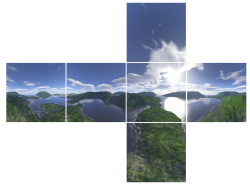
\includegraphics[width=0.5\textwidth]{images/skybox.png}
\caption{Exemplo de um textura para skybox.}
\end{center}
\end{figure}

\section{Sound}
Digamos que a experiência agradavel de um jogo nao esta apenas na visão. O som é também importante. Como tal acrescentamos este extra ao jogo, conseguindo-o através da biblioteca openAL. Na primeira etapa entregamos apenas alguns sons e uma musica  de fundo, nesta etapa, munidos dos clássicos sons da famosa personagem \textit{Super Mario}, fazemos o jogo ganhar outro significado, existe assim som para o salto, para a perda de vida, para o "ganhar o jogo", para o "perder o jogo" e de fundo.


\section{Vidas}
O conceito do jogo é simples, existem chaves, existe um local final, existem torres e existem balas. Como tal optamos por colocar "vidas", digamos que o jogador começa com um determinado número de vidas, perdendo uma por cada vez que é atingido por uma bala.

\begin{figure}[here]
                 \centering{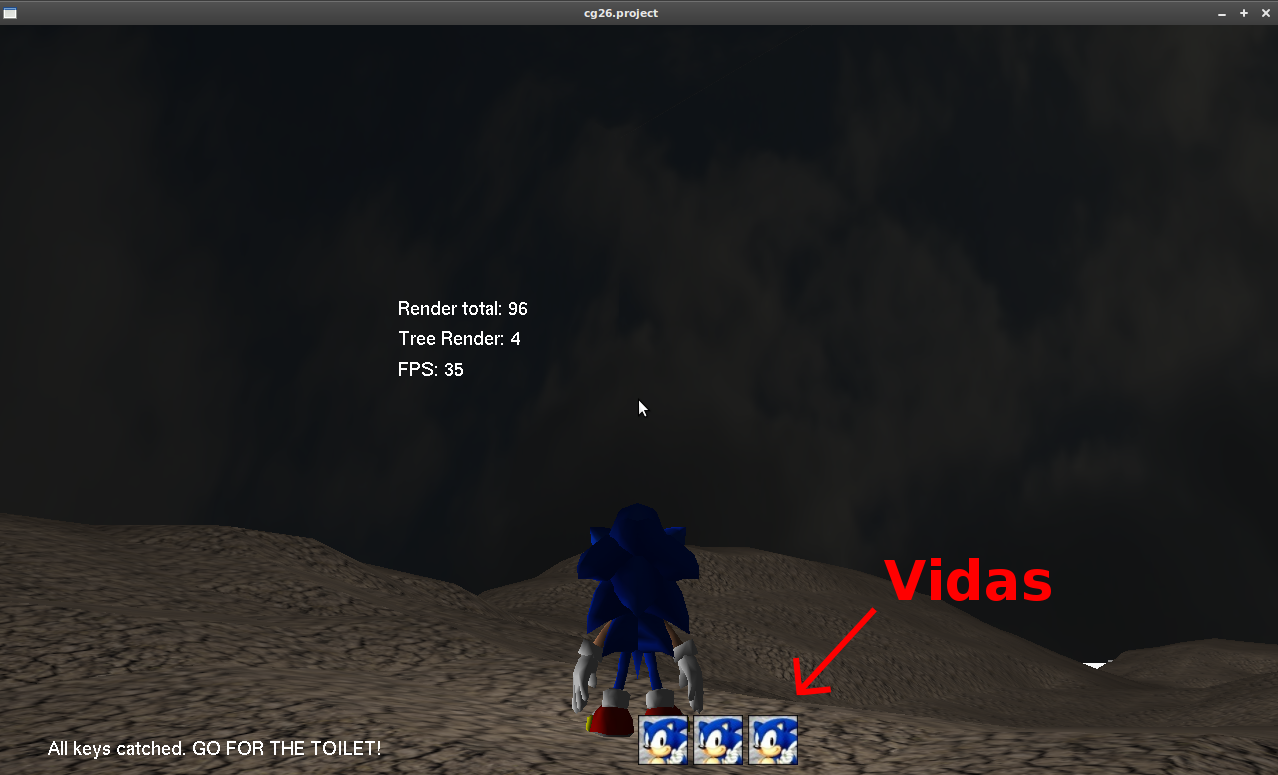
\includegraphics[width=0.8\textwidth]{images/lifes.png}}
                 \caption{Screenshot para as vidas.}
                 \label{fig:prototype}
\end{figure}


\section{Colisões}
Para aumentar o nível de realismo do jogo, decidimos implementar um sistema de colisões entre o jogador e as torres e árvores, para impedir que este se aproxime demasiado e as atravesse.

As colisões foram implementadadas à custa da seguinte função:

\begin{lstlisting}[caption=Cálculo de colisões]
void Player::calcColisions() {
	//colisoes com as torres
	for (int i = 0; i < g_towers->num_towers; i++) {
		float dist = this->coords->horizontalDistance(g_towers->towers[i]->coords);
		if (dist < tower_colision_dist) {
			float ang = g_towers->towers[i]->ang_x;
			coords->x = (g_towers->towers[i]->coords->x + tower_colision_dist * cos(-ang));
			coords->z = (g_towers->towers[i]->coords->z + tower_colision_dist * sin(-ang));
		}
	}
	
	//colisoes com as arvores
	for (int i = 0; i < g_trees->num_trees; i++) {
		float dist = this->coords->horizontalDistance(g_trees->trees[i]->coords);
		if (dist < tree_colision_dist) {
			Vertex *direction = g_trees->trees[i]->coords->directionVector(this->coords);
			//direction->x = -direction->x;
			//direction->z = -direction->z;
			float ang = acos(direction->x / dist);
			if (this->coords->z <= g_trees->trees[i]->coords->z)
				ang = -ang;
			coords->x = (g_trees->trees[i]->coords->x + tree_colision_dist * cos(-ang));
			coords->z = (g_trees->trees[i]->coords->z + tree_colision_dist * sin(ang));
		}
	}
}
\end{lstlisting}

A colisão apenas faz com que, quando o jogador entra num determinado raio de uma árvore ou torre, é empurrado para fora, na direcção dada pelo angulo entre a torre/árvore e o jogador.
Um aspecto importante a ter é conta é a altura em que esta função é invocada.
Inicialmente era chamada no update do jogador, mas isto fazia com que o jogador bloqueasse sempre que fosse contra uma torre, sendo depois necessário recuar um bocado.
Para resolver este problema, passou-se a fazer a detecção de colisões também depois do update das torres. Desta forma, é permitido que o angulo das torres seja actualizado, durante o seu update, e assim a direcção para a qual o jogador é empurrado já tem em conta o novo angulo, fazendo com que, ao avançar em direcção a uma torre, o jogador automaticamente a contorne.


\section{Salto}
Um extra que foi relativamente fácil de implementar foi permitir que o jogador salte.
Isto foi feito com recurso ao seguinte código acrescentado à função de update do jogador:

\begin{lstlisting}
if (space == KEY_ON && !isJumping && canJump) {
		isJumping = true;
		jump_time = 0;
		Sound::play(SOUND_JUMP);
	}

	if (isJumping) {
		jump_time++;
		//coords->y += jumpOff(jump_time) - jumpOff(jump_time - 1);
		coords->y += jumpOff(jump_time);
		if (anim->get_anim() != MOVE_JUMP)
			anim->set_anim(MOVE_JUMP);

		float max_height = g_map->triangulateHeight(coords->x, coords->z);
		if (coords->y < max_height) {
			coords->y = max_height;
			isJumping = false;
			anim->set_anim(MOVE_NONE);
			canJump = false;
			glutTimerFunc(jump_cooldown, GLManager::allowPlayerJump, 0);
		}

	} else if (isMoving()) {
		coords->y = g_map->triangulateHeight(coords->x, coords->z);
		if (anim->get_anim() != MOVE_WALK)
			anim->set_anim(MOVE_WALK);

	} else {
		anim->set_anim(MOVE_NONE);
	}
\end{lstlisting}

A função de salto é a seguinte:

\begin{lstlisting}
float Player::jumpOff(int off) {
	return -0.1 * off + 2;
}
\end{lstlisting}

Esta função corresponde à derivada da função de salto idealizada para o jogador. Assim para cada instante sabe-se o incremento a dar à altura do jogador durante o tempo em que este está a saltar.


\section{Iluminação}
Para a iluminação do jogo, foi idealizada uma luz posicionada nas coordenadas do jogador, e com uma intensidade mais fraca que a luz pré-definida. Isto cria um efeito mais sombrio e realista do que a utilização de uma luz uniforme em todo o mapa.

Um dos aspectos mais importantes a ter em conta para a iluminação foi em relação às árvores. Cada árvore é constituida por dois quadrados, mas cada um deles tem uma orientação definida através da sua normal.
Por pré-definição, a iluminação é feita apenas sob as faces frontais de cada poligono, o que faria com que, para cada uma das 4 faces de uma árvore, duas delas não seriam iluminadas.

Para resolver este problema surgiram duas alternativas: utilização de 4 texturas por árvore, cada uma com uma orientação diferente, em vez de apenas duas com a opção GL\_CULL\_FACE desligada para ser desenhada de ambos os lados. Ou em alternativa, a utilização da opção do OpenGL \textbf{glLightModelf(GL\_LIGHT\_MODEL\_TWO\_SIDE, 1)}

Para decidir sobre uma destas implementações, foi utilizado o Profiling, e foram medidos, para cada uma das alternativas, o tempo de render das árvores e o tempo de render total da cena.

De notar que, para serem obtidos números relevantes, foi necessário aumentar o número de árvores para 10000.
Eis os resultados:
\begin{itemize}
\item 2 texturas por árvore, opção GL\_LIGHT\_MODEL\_TWO\_SIDE:
	\begin{itemize}
		\item[render das árvores] 33 ms;
		\item[render total]	49 ms;
		\item[FPS] 20.
	\end{itemize}
\item 4 texturas por árvore, iluminação pré-definida:
	\begin{itemize}
		\item[render das árvores] 85 ms;
		\item[render total]	70;
		\item[FPS] 10. 
	\end{itemize}
\end{itemize}

Como se pode constatar, a primeira opção é claramente a mais eficiente, e portanto foi a solução escolhida.


\section{Game Mode}
Foi adicionado no ficheiro \textbf{config.ini} uma opção fullscreen, que permite correr o jogo em GameMode. Isto é uma capacidade do OpenGL de correr o jogo usando o ecrã completo e com algumas caracteristicas especiais que permitem criar um ambiente mais apropriado para se jogar.

O código a acrescentar foi simples, bastando, na inicialização, calcular o tamanho do ecrã para fornecer como parametro à função \textbf{glutGameModeString} e depois activar o GameMode caso a opção esteja activa:

\begin{lstlisting}[caption=Activação do Game Mode]
	void initGameMode() {
		stringstream stream;
		stream << glutGet(GLUT_SCREEN_WIDTH) << 'x' << glutGet(GLUT_SCREEN_HEIGHT) <<
			':' << conf.rint("window:def_window_depth") << '@' << conf.rint("window:def_refresh_rate");

		glutGameModeString(stream.str().c_str());
		if (conf.rint("window:fullscreen") && glutGameModeGet(GLUT_GAME_MODE_POSSIBLE))
			glutEnterGameMode();
	}
\end{lstlisting}


\newpage

% ------------------ CONCLUSAO
\chapter{Conclusão}
Apenas a experiência terá algo a acrescentar. Terminamos assim com algo cuja imagem fala por si, um conceito simples, aos requisitos acrescentamos as árvores, de referir também as colisões com árvores e torres, a possibilidade de saltar, e assim evitar as balas, o céu, as animações, as imagem das vidas, o full screen, isto, em termos de jogo, em termos de implementação contamos com o documento de configuração \textit{.ini}, o md2loader, profilling, entre outros.

%\chapter*{Bibliografia}

\chapter{Referências}
\textbf{Livros}
\begin{itemize}
\item{"OpenGL Programming Guide", Woo, Neider, Davis and Schneider, Addison Wesley}
\end{itemize}


\textbf{Sites}
\begin{itemize}
\item{www.lighthouse3d.com, acedido em Maio 2010}
\item{www.opengl.org, acedido em Maio 2010}
\item{www.gamasutra.com, acedido em Maio 2010}
\end{itemize}


\appendix
\chapter{Código fonte}


\end{document}
  
